\begin{subfigure}{0.4\textwidth}
    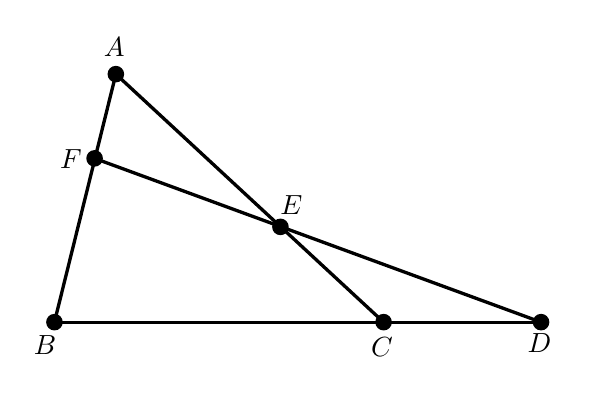
\begin{tikzpicture}[scale = 1]
        \clip(-1.12,1.19) rectangle (5.78,5.6);
        \draw [line width=1.2pt] (0,5.01)-- (3.4,1.86);
        \draw [line width=1.2pt] (-0.78,1.86)-- (0,5.01);
        \draw [line width=1.2pt] (-0.78,1.86)-- (5.4,1.86);
        \draw [line width=1.2pt] (5.4,1.86)-- (-0.27,3.94);
        \begin{scriptsize}
            \normalsize
            \fill [color=black] (0,5.01) circle (3.0pt);
            \draw[color=black] (-0.02,5.36) node {$A$};
            \fill [color=black] (-0.78,1.86) circle (3.0pt);
            \draw[color=black] (-0.9,1.57) node {$B$};
            \fill [color=black] (3.4,1.86) circle (3.0pt);
            \draw[color=black] (3.38,1.55) node {$C$};
            \fill [color=black] (5.4,1.86) circle (3.0pt);
            \draw[color=black] (5.38,1.59) node {$D$};
            \fill [color=black] (2.09,3.07) circle (3.0pt);
            \draw[color=black] (2.23,3.35) node {$E$};
            \fill [color=black] (-0.27,3.94) circle (3.0pt);
            \draw[color=black] (-0.57,3.93) node {$F$};
        \end{scriptsize}
    \end{tikzpicture}
\end{subfigure}
\hspace{0.1\textwidth}
\begin{subfigure}{0.4\textwidth}
    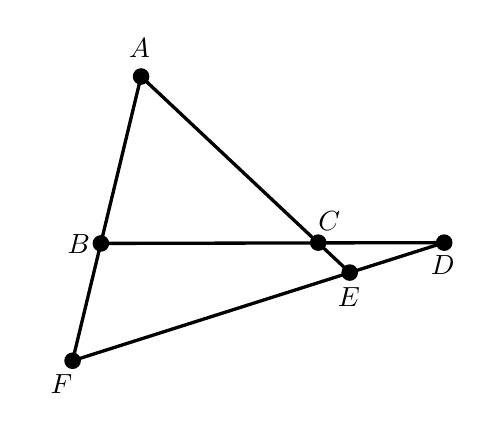
\begin{tikzpicture}[scale = 1]
        \clip(-0.12,0.2) rectangle (5.47,5.01);
        \draw [line width=1.2pt] (1.32,4.39)-- (3.97,1.9);
        \draw [line width=1.2pt] (0.45,0.78)-- (1.32,4.39);
        \draw [line width=1.2pt] (0.45,0.78)-- (5.17,2.28);
        \draw [line width=1.2pt] (5.17,2.28)-- (0.81,2.27);
        \begin{scriptsize}
            \normalsize
            \fill [color=black] (1.32,4.39) circle (3.0pt);
            \draw[color=black] (1.3,4.75) node {$A$};
            \fill [color=black] (0.45,0.78) circle (3.0pt);
            \draw[color=black] (0.31,0.48) node {$F$};
            \fill [color=black] (3.97,1.9) circle (3.0pt);
            \draw[color=black] (3.96,1.59) node {$E$};
            \fill [color=black] (5.17,2.28) circle (3.0pt);
            \draw[color=black] (5.15,2) node {$D$};
            \fill [color=black] (3.57,2.28) circle (3.0pt);
            \draw[color=black] (3.71,2.56) node {$C$};
            \fill [color=black] (0.81,2.27) circle (3.0pt);
            \draw[color=black] (0.53,2.26) node {$B$};
        \end{scriptsize}
    \end{tikzpicture}
\end{subfigure}